% !Mode:: "TeX:UTF-8"
\chapter{目标检测与多目标跟踪}
\label{technologies}
本工作主要涉及到目标检测与多目标跟踪领域,相关技术原理比较多。在详细介绍本工作主要内容之前,有必要单独使用一章内容介绍目标检测与多目标跟踪的相关技术原理,为下一章DODT模型的介绍提供技术参考。

\section{目标检测}
\label{object_detection}
目标检测 (Object Detection) 作为计算机视觉中最基本的任务之一,一直以来都受到了学术界与产业界的密切关注。 特别是在最近二十多年,随着深度学习技术的飞速发展, 神经网络已经是目标检测中必不可少的组成部分。 可以说,是深度学习的引入将目标检测推向了新的高度, 使其性能远远超出了传统方法。 以图像数据为例, 目标检测需要在图片中精确找出物体所在的位置 (一般以矩形框出),并标注物体的类别。由于物体的尺寸变化范围很大,摆放物体的角度、姿势等也不确定,并且物体间也会有重叠,这些问题使得目标检测问题并不是那么容易解决。现阶段基于深度学习的目标检测框架主要有两类, 一类是以 Faster-RCNN\cite{ren2015faster} 为代表的两阶段目标检测方法, 另一类是以 YOLO\cite{redmon2016you} 为代表的单阶段目标检测方法。 本小节将详细介绍这两种框架的发展历史、框架结构与实现原理, 此外,本小节也将简单介绍三维目标检测与二维目标检测的差异。

\subsection{两阶段目标检测}
\label{two-stage}
目标检测任务包含目标识别以及目标定位两个子任务, 一般的实现思路是先用区域提取算法截取图像中可能是目标的区域(候选区域),然后分别送入分类器进行分类,以及进行坐标回归获得更加精确的目标边界框。 将候选区域提取任务与后续分类回归任务分开,这就是两阶段物体检测的实现思路。 两阶段物体检测算法的代表是R-CNN系列工作,该系列历经 R-CNN\cite{6909475},Fast-RCNN\cite{girshick2015fast} 再到 Faster-RCNN\cite{ren2015faster}, 将两阶段物体检测框架不断完善,成为该领域中的经典。 

\subsubsection{发展历程}
R-CNN可以说是利用深度学习技术进行目标检测的开山之作。 该工作使用选择性搜索(Selective Search)算法\cite{UijlingsSelective}代替传统的滑动窗口来提取候选区域, 并且利用神经网络对图片进行特征提取,然后利用提取的特征回归更加精确的边界框,同时使用SVMs进行类别判断。该工作奠定了两阶段目标检测框架的基本结构,即一个区域提取(Region Proposal)算法用于提取输入图像中可能是目标的区域, 一个CNN网络用于提取区域特征,一个分类算法用于类别鉴定以及一个回归模型用于回归出精确的物体边界框。2015年,在R-CNN的基础上,RBG(Ross B. Girshick) 又提出了Fast-RCNN算法。该算法借鉴了SPP-Net\cite{7005506}的实现,对R-CNN做了改进,使得检测性能进一步提高,其结构如 \figurename \, \ref{fig:fast-rcnn}所示。具体而言有两个重大改进:(1)将候选区域提取阶段移到了图像特征提取之后,即只对原图做一次卷积,然后在特征图上运行候选区域提取算法得到候选区域特征图,然后将每一个特征图输入RoI(region of interest)层来将不同尺度的特征图转化为相同维度的特征向量,之后送入全连接层进行后续处理;(2)R-CNN训练神经网络提取图像特征,之后用支持向量机进行分类以及用一个回归模型精修边界框。而Fast-RCNN则利用两个全连接层(一个分类分支与一个回归分支) 将分类与回归任务整合到一个模型里联合训练,这为之后的目标检测端对端训练打下了基础。

\begin{figure}[!t]
	\centering
	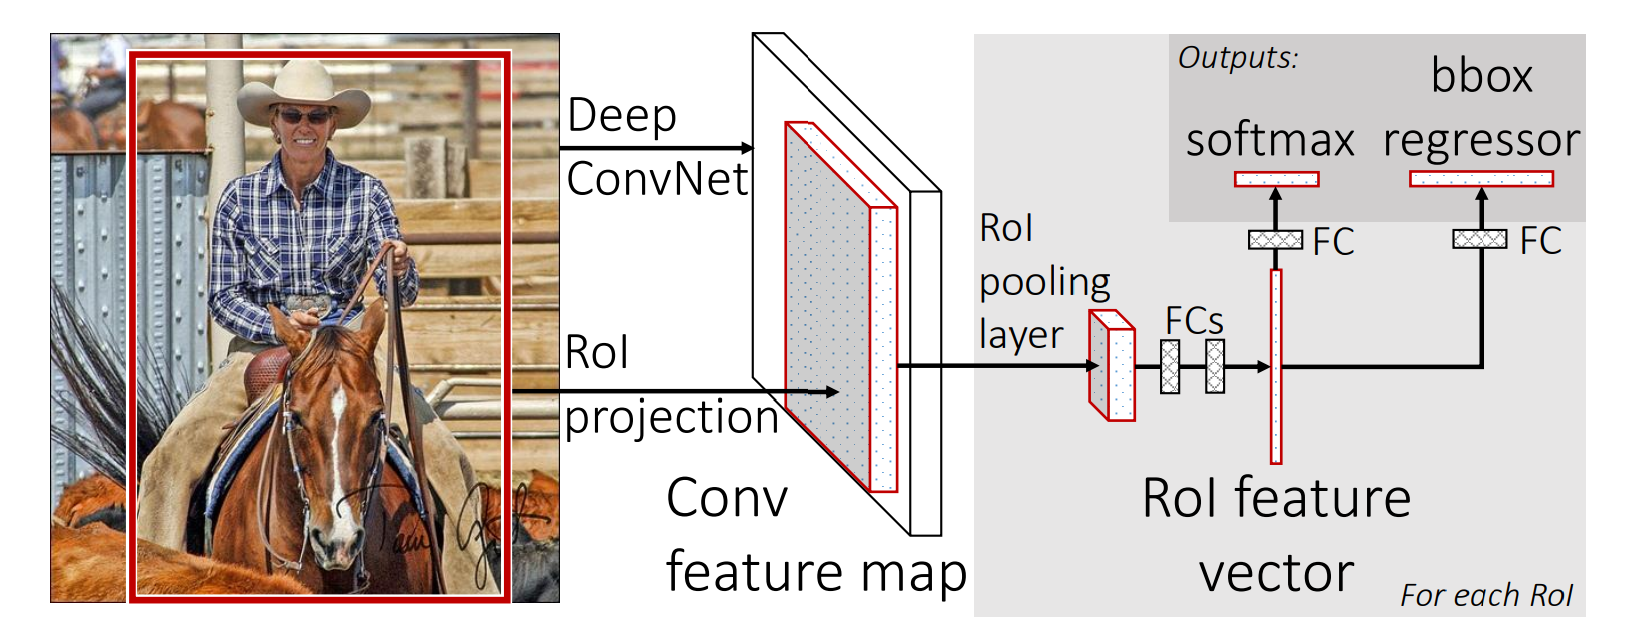
\includegraphics[width=0.95\textwidth]{./imgs/fast-rcnn.png}
	\caption{Fast-RCNN 结构示意}
	\label{fig:fast-rcnn}
\end{figure}


尽管Fast-RCNN 相对于 R-CNN 已经提速了不少,但要实现实时检测,网络测试时运行速度还是不够,其中主要的瓶颈是候选区域提取阶段十分耗时。基于CPU实现的 Selective Search 算法提取一幅图像的所有候选区域(Proposals)需要约2s时间,效率更高的 EdgeBoxes\cite{Zitnick2014Edge} 算法虽然在一定程度上提高了候选区域提取的准确率和速度,但处理一幅图像仍然需要0.2s。为了解决这个问题,2015年微软亚洲研究院提出了Faster-RCNN算法,该算法引入了候选区域提取网络(Region Proposal Network,RPN),使用神经网络取代传统的区域提取算法,将单幅图像候选区域提取时间缩短到了10ms。下一小节将以Faster-RCNN为代表,重点介绍两阶段物体检测框架的结构以及实现细节。

\subsubsection{Faster-RCNN框架结构}

\begin{figure}[!t]
	\centering
	\begin{minipage}[t]{0.4\textwidth}
		\centering
		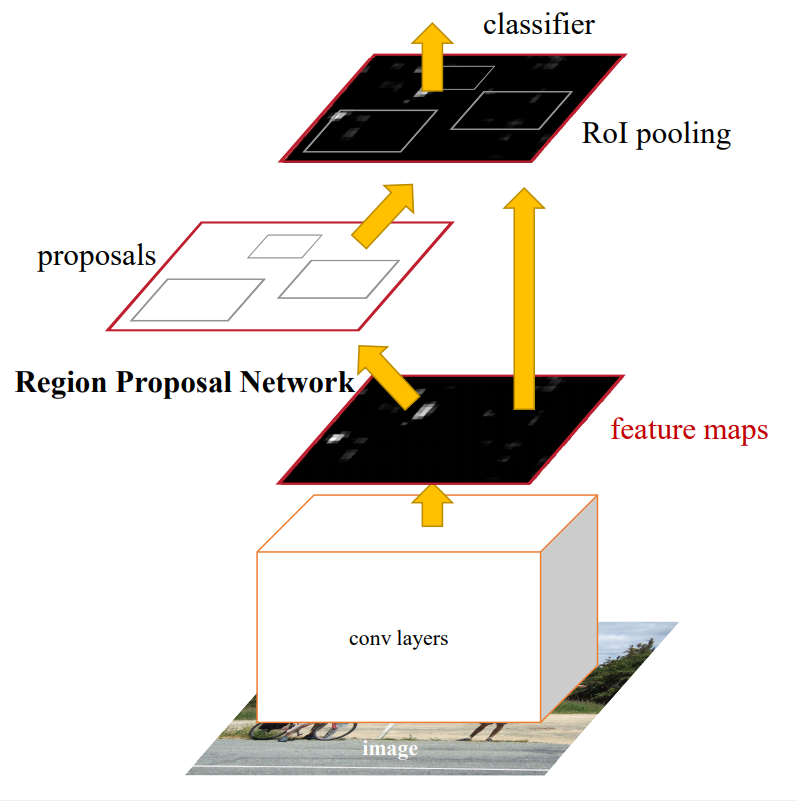
\includegraphics[width=\textwidth]{./imgs/faster-rcnn.png}
		\caption{Faster-RCNN 结构示意}
		\label{fig:faster-rcnn}
	\end{minipage}
	\begin{minipage}[t]{0.58\textwidth}
		\centering
		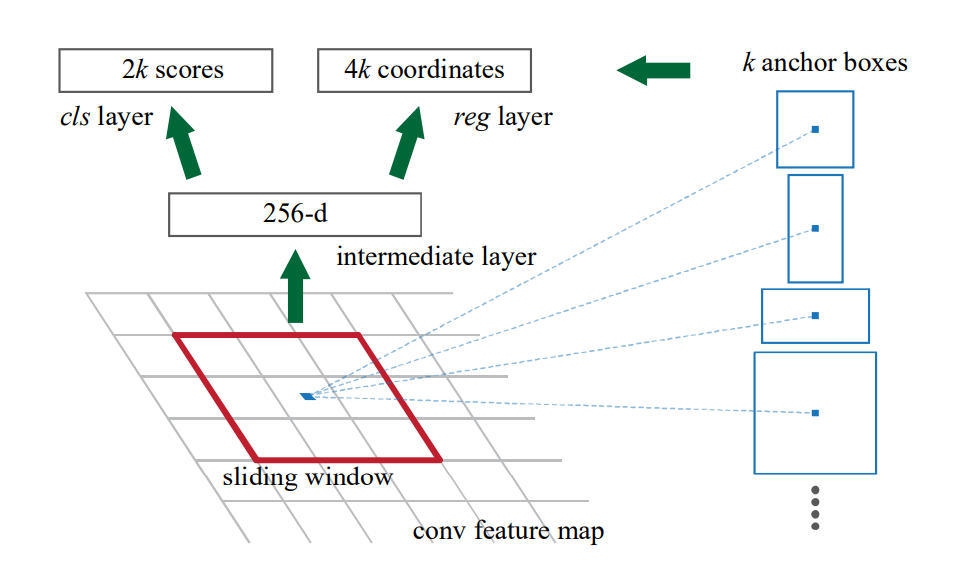
\includegraphics[width=\textwidth]{./imgs/rpn.png}
		\caption{RPN 结构示意}
		\label{fig:rpn}
	\end{minipage}
\end{figure}


Faster-RCNN框架由两大模块组成,候选区域提取模块(RPN)和检测模块, 如 \figurename \, \ref{fig:faster-rcnn} 所示。其中RPN取代了原来的区域提取算法,而检测模块和Fast-RCNN类似,都是由卷积层以及全连接层组成。对于Faster-RCNN网络,首先输入一幅图像,图像经过卷积神经网络提取特征得到特征图(feature maps),然后特征图输入到RPN模块预测得到候选框(proposals),之后根据候选框去特征图中截取相应的特征块。这时的特征块由于尺寸不一样(为了满足物体的尺度多样性,候选框的尺寸不一样),不能直接输入到检测模块进行分类和回归,而是要通过RoI池化操作得到相同尺寸的特征向量,然后送入检测分支(classifier)和回归分支(regressor)分别预测得到分类结果以及预测框的信息。RPN是Faster-RCNN新引进的模块,其原理如\figurename \, \ref{fig:rpn}所示。在特征提取网络生成的特征图($M \times N$)上,使用$k$ 个 $n \times n$ 的卷积核卷积生成$M \times N \times k$个维度为256的中间特征向量,之后输入分类全连接层(cls layer)和回归全连接层(reg layer),分别用来预测候选框的类别(前景/背景,$M \times N \times 2 \times k$)以及候选框的位置信息(中心点坐标$x, y$以及宽高$w, h$, 整体维度为$M \times N \times 4 \times k$)。其中,$k$ 也可以表示为对于特征图上的每一个像素点(或者成为锚点),都负责预测$k$个锚点框(anchor boxes)。另外,为满足候选框的尺寸变化,这$k$个锚点框会设置不同的尺寸和长宽比。原始的Faster-RCNN中设置了三种不同的尺寸:$128\times 128$,$256 \times 256$, $512 \times 512$(px), 也设置了三种不同的长宽比:$1:1$, $1:2$, $2:1$。因此 $k = 3 \times 3 = 9$,意味着每个锚点负责预测9个不同的候选框。

\subsubsection{Faster-RCNN网络训练}
构建好了网络结构,网络的训练还需要准备训练数据,明确损失函数等。目标检测的训练数据一般有公开的数据集,如COCO\footnote[5]{http://cocodataset.org/},PASCAL\footnote[6]{http://host.robots.ox.ac.uk/pascal/VOC/}等,然而Faster-RCNN还需额外训练RPN网络,因此需要额外准备RPN网络训练的标签数据。候选框标签的生成需要借助真实标签数据:首先根据上文提到的锚点的概念,以特征图尺寸为参照生成$M \times N \times k$个候选框(一共有$M \times N$个锚点,每个锚点有$k$个不同尺寸的锚点框),然后根据候选框与真实物体框的重叠程度(一般以候选框与真实框的交并比IoU为量化指标)计算每个候选框的得分。候选框的得分可作为其划分前景类还是背景类的依据,譬如得分大于0.65划分为前景,小于0.35划分为背景,而得分在[0.35,0.65]之间的候选框则忽略不计,这样就得到了训练RPN网络的标签数据。

Faster-RCNN的损失函数由两部分构成,RPN损失和Fast-RCNN损失,并且这两部分损失又都包括两类损失,分类损失和回归损失。
\begin{equation}
L(\{p_i\},\{t_i\}) =\frac{1}{N_{cls}} \sum_{i}L_{cls}(p_i, p^*_i) + \lambda \frac{1}{N_{reg}} \sum_{i} p^*_i L_{reg}(t_i,t^*_i)
\label{con:rpn_loss}
\end{equation}
RPN损失函数如公式 \ref{con:rpn_loss} 所示,其中第一部分为分类损失,第二部分为回归损失。分类损失计算了RPN预测生成的候选框类别的交叉熵损失$L_{cls}$, 其公式如 \ref{con:cross_entropy}所示。其中$p_i$为预测生成的候选框类别,$p^*_i$是标签值。RPN网络生成的候选框分为前景和背景,前景标签为1,背景为0,是一个二分类问题。
\begin{equation}
L_{cls} = -\log[p^*_ip_i + (1-p^*_i)(1-p_i)]
\label{con:cross_entropy}
\end{equation}
在训练中,RPN网络生成的$M \times N \times k$个候选框,然而并不是每个候选框都会纳入损失值的计算范围,因为这些候选框有很多会重叠在一起。Faster-RCNN使用了非极大值抑制(Non-Maximum Suppression,NMS)算法进行初步筛选,减少重叠的候选框。NMS算法详细流程如算法 \ref{alg:nms} 所示:对于RPN生成的候选框集合 $\mathcal{B}$以及对应的置信度集合$\mathcal{S}$,首先选择对应最大置信度的候选框$M$,将其从$\mathcal{B}$中移除并加入最终候选框集合$\mathcal{D}$;然后遍历$\mathcal{B}$,移除与$M$的交并比(Intersection of union, IoU)大于阈值$\epsilon$的框;重复此过程,直到$\mathcal{B}$为空。通过选择合适的阈值(Faster-RCNN中为0.7),NMS算法可以过滤掉大部分重叠的候选框,之后从中随机选取$N_{cls}$个候选框计算分类损失,在Faster-RCNN中$N_{cls} = 256$。
\begin{algorithm}[t]
	\caption{非极大值抑制算法}
	\label{alg:nms}
	\textbf{输入: } $\mathcal{B}=\{b_1,...,b_N\}$,RPN生成候选框集合; $\mathcal{S}=\{s_1,...,s_N\}$, 生成候选框对应的置信度集合; $\epsilon$, 置信度阈值 \\
	\textbf{初始化:} $\mathcal{D} \leftarrow$ \{ \},最终候选框集合 \\
	\While{$\mathcal{B} \neq \emph{empty }$}{
		$m \leftarrow \emph{argmax } \mathcal{S}$ \\
		$\mathcal{M} = b_m$ \\
		$\mathcal{D} \leftarrow \mathcal{D} \bigcup \mathcal{M}; \, \mathcal{B}  \leftarrow\mathcal{B} - \mathcal{M}$ 
	 
		\For{$b_i \emph{ in } \mathcal{B}$}{
			\If{$\emph{IoU}(\mathcal{M},b_i) \leq \epsilon$}{
				$\mathcal{B} \leftarrow \mathcal{B} - b_i; \, \mathcal{S} \leftarrow \mathcal{S} - s_i$
			}
		}
	}
	\textbf{输出: } $\mathcal{D},\mathcal{S}$
\end{algorithm}

RPN回归损失计算预测候选框的$Smooth_{L1}$损失$L_{reg}$,注意到RPN回归损失只计算前景的损失,因此$L_{reg}$前需乘以$p^*_i$(前景为1,背景为0)。$N_{reg} = N_{cls}$,为经过NMS算法过滤后随机选择的候选框数。$Smooth_{L1}$损失公式如\ref{con:smooth_l1}所示,
\begin{equation}
L_{reg}(t_i,t^*_i) = 
\begin{cases}
0.5(t_i-t^*_i)^2 & |t_i-t^*_i| \leq 1 \\
|t_i-t^*_i| - 0.5 & \text{否则}
\end{cases}
\label{con:smooth_l1}
\end{equation}
其中 $t_i$和$t^*_i$分别对应预测候选框以及真实候选框的信息。其中$t_i = (t^x_i, t^y_i,t^w_i,t^h_i)$ 为一四维偏移向量,其计算公式如\ref{con:offsets}所示。其中$(x_a,y_a,w_a,z_a)$分别是对应锚点框中心点坐标以及宽高。从损失值的计算可以看出,RPN并不直接回归出候选框的位置信息,而是回归候选框与对应的锚点框的偏移量,这种处理有利于稳定网络的训练过程,也有利于网络的收敛。
\begin{equation}
t_x = \frac{x - x_{a}}{w_{a}}; \, t_y = \frac{y - y_{a}}{h_{a}}; \,
t_w = \log(\frac{w}{w_{a}}); \, t_h = \log(\frac{h}{h_{a}})
\label{con:offsets}
\end{equation}

检测模块的Fast-RCNN的损失和RPN类似,同样由分类损失和回归损失组成。不过RPN的分类损失是二分类的交叉熵损失,而Fast-RCNN的分类损失是多分类的交叉熵损失,不过将类别标签转化为one-hot向量后并没有本质区别。和RPN类似,Fast-RCNN也不针对所有预测框计算损失,而是先通过更严格的NMS算法(Faster-RCNN中阈值设置为0.3)筛选出一批重叠度低、得分高的预测框,然后随机选择一定数量的预测框进行损失值计算。Fast-RCNN的回归损失基本也和RPN的一致,也不直接回归真实框的位置信息,而是回归物体真实框与锚点框的偏移量,偏移量的编码方式与上文RPN中的类似。

\subsection{单阶段目标检测}
\label{one-stage}
从 RCNN 到 Fast-RCNN 再到 Faster-RCNN,一直采用先计算出候选区域然后再在候选区域上进行检测的设计范式。该模式可以获得很好的检测精度,然而在速度上还不佳,最好的Faster-RCNN只能达到0.2s一帧的检测速度,离实时检测还有较大差距。单阶段目标检测提供了另一种更直接的设计思路:不显式计算候选框,而是通过神经网络直接预测物体的位置与类别。该模式的代表工作有YOLO系列以及SSD,本节以YOLO为例,介绍单阶段目标检测的实现方法以及网络训练。


\begin{figure}[!t]
	\centering
	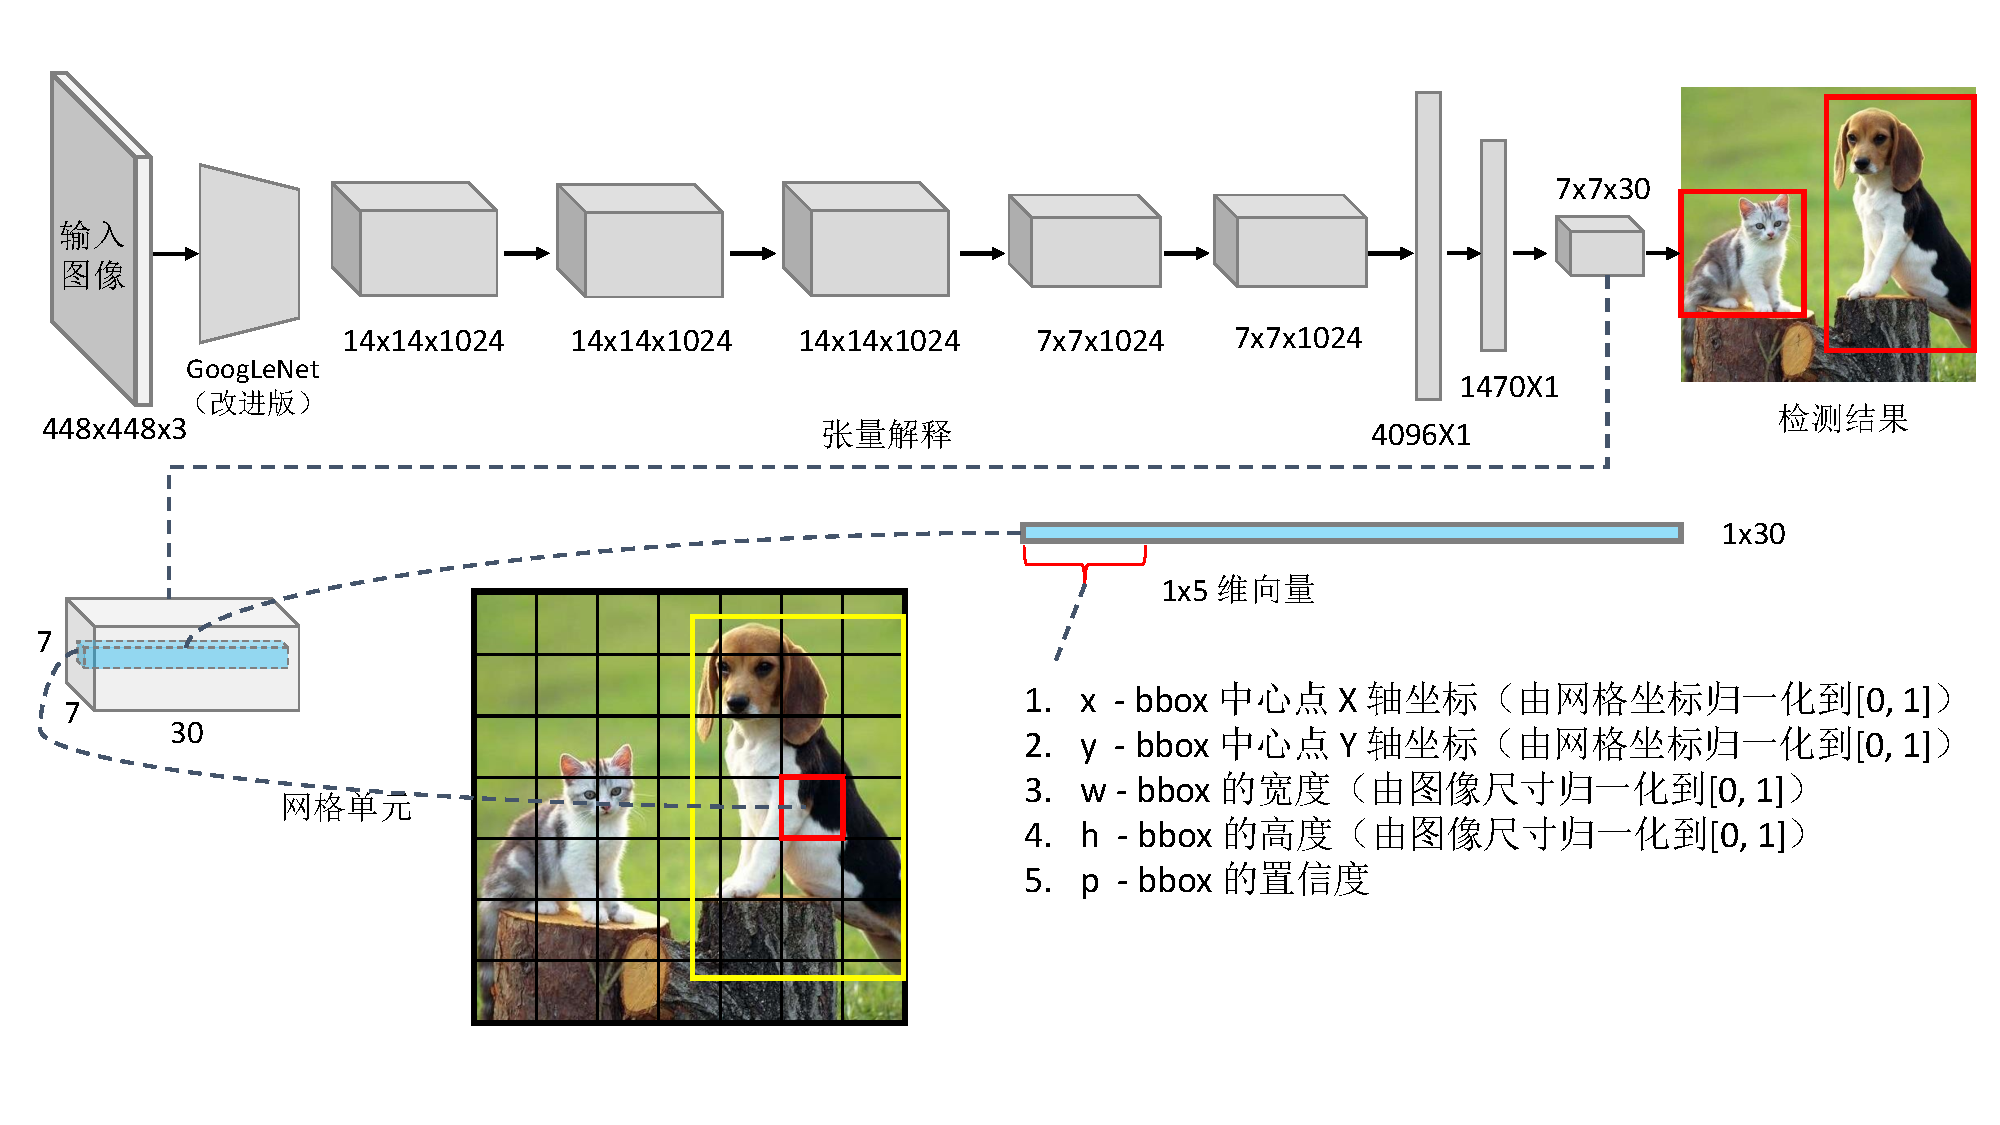
\includegraphics[trim={0.5cm, 2cm, 0cm, 1cm}, clip,width=\textwidth]{./imgs/yolo.pdf}
	\caption{YOLO结构示意图。}
	\label{fig:yolo}
\end{figure}


YOLO的整体架构如\figurename \, \ref{fig:yolo}所示。与RCNN系列工作不同,YOLO将目标检测作为回归任务来解决。YOLO首先将输入图像宽高调整到$448 \times 448$,然后输入到由GoogLeNet改进的网络中,最后输出一个维度为$S \times S \times (B \times 5 + C)$的张量$\mathcal{T}$。$\mathcal{T}$可以这么理解,首先将一幅图像分成$S \times S$ (YOLO是$7\times 7$)个网格,对于每个网格$s$,其对应着$\mathcal{T}$中的一项维度为$1 \times (B \times 5 + C)$的向量$t$。如果一个目标物体的中心落在$s$上,则$s$负责预测该物体,预测结果编码在向量$t$中。$t$维度为$B \times 5 + C$,其中 $B$ 表示每个网格预测两个边界框(bounding box, bbox);$5$编码了bbox的信息,分别是$(x,y,w,h,c)$,代表bbox中心点坐标、宽高以及置信度;$C$ 表示需要预测C个类,每个值表示预测为该类的概率值$Pr(class_i|object)$。

和Faster-RCNN类似,YOLO也不是直接回归出物体的实际坐标和宽高,而是bbox相对于单元格的偏移量。对于向量$t=(x,y,w,h,c)$,$(x,y)$的计算公式如\ref{con:yolo_xy}所示,其中$(x_c,y_c)$是bbox中心点的实际坐标,$(w_i, h_i)$是图像的宽高,$x_{col}, y_{col}$是单元格的坐标。最终预测出来的$(x,y)$是经过归一化处理的,中心相对于单元格的偏移。$(w,h)$的计算公式如\ref{con:yolo_wh}所示,是bbox相对于整张图像的比例。置信度$c$的计算公式如\ref{con:yolo_c}所示,由两部分组成,$Pr(object)$表示单元格内是否有物体,有为1,没有则为0;$IoU^{Truth}_{Pred}$表示bbox位置的准确度,用IoU衡量。
\begin{gather}
x = \frac{x_c}{w_i}S - x_{col}; \, y = \frac{y_c}{h_i}S - y_{row} 
\label{con:yolo_xy}\\
w = \frac{w_b}{w_i}; \, h = \frac{h_b}{h_i}
\label{con:yolo_wh}\\
c = Pr(object)*IoU^{Truth}_{Pred}
\label{con:yolo_c}
\end{gather}

在测试阶段,网络最终输出为一个$S \times S \times (B \times 5 + C)$,其中包含$S \times S \times B$个预测框,每个预测框的最终概率为 $Pr(class_i|object) * c$,为综合了定位误差和分类误差的20维向量。最后这$S \times S \times B \times C$ 列的结果送入NMS算法去除重复的检测框,得到最终的检测结果。

YOLO的损失函数设计比较复杂,如公式\ref{con:yolo_loss}所示。YOLO的损失函数都采用平方和损失,可分为五部分来看:
\begin{equation}
\begin{split}
L_{yolo} &= \lambda_{coord} \sum^{S^2}_{i=0} \sum^{B}_{j=0} \mathds{1}^{obj}_{i,j} (x_i - \hat{x}_i)^2 + (y_i - \hat{y}_i)^2 \\
&+ \lambda_{coord} \sum^{S^2}_{i=0} \sum^{B}_{j=0} \mathds{1}^{obj}_{i,j} \left(\sqrt{w_i} - \sqrt{\hat{w}_i}\right)^2 + \left(\sqrt{h_i} - \sqrt{\hat{h}_i}\right)^2 \\
&+ \sum^{S^2}_{i=0} \sum^{B}_{j=0} \mathds{1}^{obj}_{i,j}\left(C_i -\hat{C}_i\right)^2\\
&+ \lambda_{noobj} \sum^{S^2}_{i=0} \sum^{B}_{j=0} \mathds{1}^{noobj}_{i,j}\left(C_i -\hat{C}_i\right)^2\\
&+ \sum^{S^2}_{i=0}\mathds{1}^{obj}_{i}\sum_{c \in classes} \left(p_i(c) - \hat{p}_i(c)\right)^2
\end{split}
\label{con:yolo_loss}
\end{equation}
第一部分为bbox中心坐标的误差,其中$\mathds{1}^{obj}_{i,j}$表示判断第$i$个网格中第$j$个bbox是否负责预测该物体。第二部分为bbox宽高的误差,由于在对不同大小的bbox的预测中,小bbox预测偏离的容忍程度比大bbox要小很多,而平方和损失对bbox的尺度并不敏感。为了解决这个问题,YOLO使用宽高的平方根代替原来的宽高。第三部分为含有物体的bbox的置信度预测误差,第四部分为不含物体的bbox的置信度预测误差。最后一部分是对bbox类别预测的误差,其中$\mathds{1}^{obj}_{i}$表示是否有物体落在单元格$i$中。另外,为了平衡各种损失之间的比例,YOLO还加入了$\lambda_{coord}, \lambda_{noobj}$作为超参数平衡各部分损失。

YOLO由于没有显式的预测候选框的过程,因此检测速度很快。但是由于网格的设定,YOLO对相互靠的很近的物体(中心可能落在同一个单元格内),还有很小的物体检测效果不好,这是由于一个单元格只预测一个类。另外,YOLO对于同一类物体出现不常见的长宽比等情况的泛化能力较差。这些问题在其后的 YOLOv2、YOLOv3中有探究。

\subsection{三维目标检测}
\label{3d_detection}
三维目标检测目前有两大类,一类是基于二维目标检测进行扩展到三维,一类是先进行点云语意分割,然后对分割后的每个类别的点进行聚类,之后在进行物体框的回归。直接扩展二维目标检测方法的有基于两阶段目标检测的MV3D、AVOD等,基于单阶段目标检测的VoxelNet等。在模型框架层面,这一大类的三维目标检测和二维的没有多大区别,只是需要先将三维点云编码为适合卷积的数据格式,然后将二维边框编码扩展到三维,以及损失函数做出相应的修改。具体的改动将会在下一章介绍本文方法时详细介绍。另一类先分割再回归框的方法有PointRCNN等,由于这类方法与本文方法差距较大,这里不过多介绍。


\section{目标跟踪}
\label{object_tracking}
由于本工作也涉及到一些目标跟踪方面的应用,因此本文也简单介绍下目标跟踪的一些基本知识。目标跟踪问题是指给定第一帧物体的位置,根据算法预测出后续帧中该物体的位置。根据追踪物体的数量的不同,目标追踪分为单目标追踪(Single Object Tracking, SOT)和多目标追踪(Multiple Object Tracking, MOT)。SOT与MOT虽然都属于目标跟踪,但是确实两个差别很大的研究方向。由于本工作只涉及到多目标跟踪,因此会重点介绍,而单目标跟踪只会简单叙述其基本原理。

\subsection{单目标跟踪}
\label{single_tracking}
单目标跟踪只针对单个物体进行追踪,其算法实现的基本思路如下:首先根据首帧提供的物体信息提取目标物体特征,例如灰度特征、颜色特征、纹理特征或者使用神经网络提取的视觉特征;然后基于帧间的目标运动关系,构建运动模型,经典的运动模型如均值偏移、滑动窗口、卡尔曼滤波以及粒子滤波等;之后根据运动模型确定的后续帧目标位置信息,提取该图像区域特征后输入外观模型与首帧物体特征进行对比判断;最后需要一个在线更新机制在跟踪过程中不断更新外观模型,使得模型能够捕捉目标的变化,适应长距离的跟踪。

学术界针对单目标追踪有大量的研究,如首次将相关滤波引入单目标跟踪的MOSSE\cite{bolme2010visual}以及后续在此基础上发展的KCF\cite{henriques2014high}、DSST\cite{danelljan2014accurate}、C-COT\cite{danelljan2016beyond}以及ECO\cite{danelljan2017eco}等。另外,这些年基于孪生网络的单目标追踪模型发展迅速,如首先开创端对端深度学习式相关滤波方法先河的SiamFC\cite{bertinetto2016fully},以及加入了RPN应对尺度变化的SiamRPN\cite{li2018high}以及其改进版本DaSiamRPN\cite{zhu2018distractor}等。从近几年的单目标跟踪研究可以看出,深度学习技术也在该领域也引发了技术革新。

\subsection{多目标跟踪}
\label{mot}
多目标跟踪同时对多个物体进行跟踪,相比于单目标跟踪,其实现难度更大,因此进展较为缓慢。多目标跟踪一般会涉及到目标出现、遮挡以及离开视野等复杂情况。目前学术界针对多目标跟踪的主流实现思路是基于检测的跟踪(Detection-Based Tracking),该方法要求先由一个目标检测器将每一帧的目标都检测出来,然后再使用匹配算法将不同帧的同一物体相关联。按照处理方式,多目标跟踪算法可分为在线跟踪(Online Tracking)以及离线跟踪(Offline Tracking)。在线跟踪要求算法只能根据当前帧以及之前帧的信息得出当前帧的跟踪结果,而离线跟踪允许算法利用所有帧的信息,获取全局最优解。相对于离线跟踪,在线跟踪更适合实际应用场景。例外,还有一种近似在线跟踪(Near Online Tracking)方法,该方法利用当前帧一定窗口范围内的帧的信息得出当前帧的跟踪结果,是一种折中方法,只会导致些许延迟。

目前多目标跟踪算法基本是使用现有的检测器模型得到所有帧的检测结果,然后设计数据关联算法得到多目标跟踪结果。例如SORT\cite{bewley2016simple}使用Faster-RCNN作为目标检测器得到检测结果,然后使用中心坐标、面积、长宽比等对目标进行建模,使用卡尔曼滤波预测目标的后续状态,并将预测结果与实际结果进行匹配从而得到最终结果。在此基础上,作者使用了深度卷积神经网络提取目标特征作为匹配基础改进SORT而得到DeepSORT[\cite{wojke2017simple}。此外,还有一种比较简单的,使用前后两帧各目标框的IoU进行关联的IoU Tracker\cite{bochinski2017high},该算法严重依赖于检测框的准确率。为了改善对检测结果精度的依赖,作者之后推出了改进版V-IOU Tracker\cite{bochinski2018extending},该算法加入了检测框的长程连续性特征,没有检测出的目标不再认为立即消失,而是会根据其运动趋势保持更新一定时间步长。本工作所使用的目标跟踪算法是基于V-IoU Tracker算法改进的。

多目标跟踪的性能评价指标和单目标跟踪有很大不同,当前学术界最常使用的衡量指标为CLEAR MOT\cite{bernardin2008evaluating}论文提出的多目标追踪准确度(Multiole Object Tracking Accuracy,MOTA)和多目标追踪精确度(Multiple Object Tracking Precision,MOTP)。其中MOTA的计算公式如\ref{con:mota}所示,其中$t$表示帧数,$m_t, fp_t, mme_t$分别是$t$帧时漏检、误检以及错误匹配的数量,$g_t$为$t$帧中的真实标签。从公式可以看出MOTA可以分为三部分,$\overline{m}$为漏检率,$\overline{fp}$为误检率,$\overline{mme}$为错误匹配率,这三种错误率的总和就是总错误率。MOTA直观的给出了衡量算法连续跟踪识别目标的能力,不过没有涉及到目标的检测位置精确度。
\begin{equation}
\begin{split}
MOTA & = 1 - (\overline{m} + \overline{fp} + \overline{mme})\\
& = 1 - \left(\frac{\sum_t m_t}{\sum_t g_t} + \frac{\sum_t fp_t}{\sum_t g_t} + \frac{\sum_t mme_t}{\sum_t g_t} \right)\\
& = 1 - \frac{\sum_t (m_t + fp_t + mme_t)}{\sum_t g_t}
\end{split}
\label{con:mota}
\end{equation}
另一个指标MOTP与MOTA互补,其衡量跟踪目标位置的精确度,而不衡量跟踪识别目标的能力。MOTP的计算公式如\ref{con:motp}所示,其中$t$表示帧数,$i$表示第$t$帧第$i$个目标-预测匹配对,$d^i_t$表示第$t$帧中第$i$个目标-预测匹配对的位置误差,$c_t$表示第$t$帧中总匹配对的个数。在计算MOTA和MOTP时,都是基于整个跟踪过程计算平均值的,而不是基于每一帧的结果,这是因为基于单帧计算然后再求平均会导致和直观上不同的结果。
\begin{equation}
MOTP = \frac{\sum_{i,t} d^i_t}{\sum_t c_t}
\label{con:motp}
\end{equation}

除了MOTA与MOTP,为了更好的在轨迹层面上衡量多目标追踪,学术界一般还会引入其他指标。例如多数追踪率(Mostly Tracked,MT)、多数丢失率(Mostly Lost,ML)、ID切换次数(ID-switches,IDS)、片段数(Fragmentations,FM)。其中MT目标的大部分被追踪到的轨迹占比(大于80\%),ML表示目标的大部分跟丢的轨迹占比(小与20\%),IDS为一条跟踪轨迹改变目标编号的次数,FM为真实轨迹被打断的次数。本工作使用MOTA、MOTP以及以上四种指标评估多目标跟踪算法的性能。

\section{本章总结}
\label{tech_conclusion}
本章主要介绍了本文涉及到的两个领域,目标检测与目标跟踪的基本技术原理。首先介绍了两类目标检测框架的网络结构和训练方法,其中两阶段目标检测以Faster-RCNN作为代表进行介绍,而单阶段目标检测则以YOLO为代表进行介绍。之后,本章简单介绍了单目标跟踪算法的实现思路和几种经典算法。本章最后介绍了多目标跟踪的实现方式和几种典型算法,以及多目标追踪性能的评价指标。该章的内容是为下一章中本工作方法介绍的时候提供技术参考,本章涉及到的技术原理,下章将不再深入介绍。

% 打印时插入必要的空白页
\ifprint
	\newpage
	\thispagestyle{empty}
	\mbox{}
	
	% 避免空白页影响页码编号
	\clearpage
	\setcounter{page}{10}
\fi